\documentclass{report}


\usepackage[T1]{fontenc}
\usepackage[utf8]{inputenc}
\usepackage{amsmath}


\usepackage{enumerate}

\usepackage{graphicx}
\usepackage{fancyhdr}
\usepackage{lettrine}
\usepackage{hyperref}
\usepackage{subcaption}
\usepackage{tikz}
\usepackage{cite}
\usepackage{listings}
\usepackage[nottoc, numbib]{tocbibind}
\usepackage{../assets/scripts/tex/color-env}
\usepackage[ngerman]{babel}
\usepackage[Glenn]{fncychap}
\usepackage{trfsigns}
\usepackage{amsmath,amsfonts,stmaryrd,amssymb} % Math packages

\usepackage{enumerate} % Custom item numbers for enumerations

\usepackage[ruled]{algorithm2e} % Algorithms

\usepackage[]{mdframed} % Allows defining custom boxed/framed environments


\mdfdefinestyle{info}{%
	topline=false, bottomline=false,
	leftline=false, rightline=false,
	nobreak,
	singleextra={%
		\fill[black](P-|O)circle[radius=0.4em];
		\node at(P-|O){\color{white}\scriptsize\bf i};
		\draw[very thick](P-|O)++(0,-0.8em)--(O);%--(O-|P);
	}
}

% Define a custom environment for information
\newenvironment{info}[1][Info:]{ % Set the default title to "Info:"
	\medskip
	\begin{mdframed}[style=info]
		\noindent{\textbf{#1}}
}{
	\end{mdframed}
}


\mdfdefinestyle{warning}{
	topline=false, bottomline=false,
	leftline=false, rightline=false,
	nobreak,
	singleextra={%
		\draw(P-|O)++(-0.5em,0)node(tmp1){};
		\draw(P-|O)++(0.5em,0)node(tmp2){};
		\fill[black,rotate around={45:(P-|O)}](tmp1)rectangle(tmp2);
		\node at(P-|O){\color{white}\scriptsize\bf !};
		\draw[very thick](P-|O)++(0,-1em)--(O);%--(O-|P);
	}
}

% Define a custom environment for warning text
\newenvironment{warn}[1][Warning:]{ % Set the default warning to "Warning:"
	\medskip
	\begin{mdframed}[style=warning]
		\noindent{\textbf{#1}}
}{
	\end{mdframed}
}


\usetikzlibrary{shapes}
    \usetikzlibrary{arrows}
    \usetikzlibrary{arrows.meta,topaths}
    \usetikzlibrary{bending}
    \usetikzlibrary{calc}
\title{Elektrotechnik 1 Praktikum 1}


\usepackage[
  includehead,
  headheight = 17mm,
  footskip = \dimexpr\headsep+\ht\strutbox\relax,
  tmargin = 0mm,
  bmargin = \dimexpr17mm+2\ht\strutbox\relax,
]{geometry}

\usepackage{anyfontsize}

\usepackage{xcolor}

\definecolor{DarkGreenBlue}{HTML}{264653}
\definecolor{LightGreenBlue}{HTML}{2A9D8F}
\definecolor{LightOrange}{HTML}{E9C46A}
\definecolor{DarkOrange}{HTML}{F4A261}
\definecolor{RedOrange}{HTML}{E76F51}
\definecolor{BrightRed}{HTML}{D62828}
\definecolor{DeepBlue}{HTML}{003049}

\definecolor{codegreen}{rgb}{0,0.6,0}
\definecolor{codegray}{rgb}{0.5,0.5,0.5}
\definecolor{codepurple}{rgb}{0.58,0,0.82}
\definecolor{backcolour}{rgb}{0.95,0.95,0.92}

\lstdefinestyle{code}{
    backgroundcolor=\color{backcolour},
    commentstyle=\color{codegreen},
    keywordstyle=\color{magenta},
    numberstyle=\tiny\color{codegray},
    stringstyle=\color{codepurple},
    basicstyle=\ttfamily\footnotesize,
    breakatwhitespace=false,
    breaklines=true,
    captionpos=b,
    keepspaces=true,
    numbers=left,
    numbersep=5pt,
    showspaces=false,
    showstringspaces=false,
    showtabs=false,
    tabsize=2
}

\lstset{style=code}

\pagestyle{fancy}
\fancyhead[L]{\leftmark}
\fancyhead[R]{}
\fancyfoot[L]{}
\fancyfoot[C]{\thepage}
\fancyfoot[R]{
\includegraphics[scale=0.2]{../assets/images/haw.jpg}}
\renewcommand\headrulewidth{0.5pt}


\begin{document}


\thispagestyle{empty}
\begin{tikzpicture}[overlay,remember picture]
  \thispagestyle{empty}
  \fill[black!2] (current page.south west) rectangle (current page.north east);

  \begin{scope}[transform canvas ={rotate around ={45:($(current page.north west)+(-.5,-6)$)}}]

    \shade[rounded corners=18pt, left color=DarkGreenBlue, right color=LightGreenBlue] ($(current page.north west)+(-.5,-6)$) rectangle ++(9,1.5);

  \end{scope}

  \begin{scope}[transform canvas ={rotate around ={45:($(current page.north west)+(.5,-10)$)}}]

    \shade[rounded corners=18pt, left color=LightOrange,right color=DarkOrange] ($(current page.north west)+(0.5,-10)$) rectangle ++(15,1.5);

  \end{scope}

  \begin{scope}[transform canvas ={rotate around ={45:($(current page.north west)+(0.5,-10)$)}}]

    \shade[rounded corners=8pt, right color=DarkOrange, left color=LightOrange] ($(current page.north west)+(1.5,-9.55)$) rectangle ++(7,.6);

  \end{scope}

  \begin{scope}[transform canvas ={rotate around ={45:($(current page.north)+(-1.5,-3)$)}}]

    \shade[rounded corners=12pt, left color=DeepBlue!80, right color=DeepBlue!60] ($(current page.north)+(-1.5,-3)$) rectangle ++(9,0.8);

  \end{scope}

  \begin{scope}[transform canvas ={rotate around ={45:($(current page.north)+(-3,-8)$)}}]

    \shade[rounded corners=28pt, left color=BrightRed, right color=BrightRed!80] ($(current page.north)+(-3,-8)$) rectangle ++(15,1.8);

  \end{scope}

  \begin{scope}[transform canvas ={rotate around ={45:($(current page.north west)+(4,-15.5)$)}}]

    \shade[rounded corners=25pt, left color=RedOrange, right color=DarkOrange] ($(current page.north west)+(4,-15.5)$) rectangle ++(30,1.8);

  \end{scope}

  \begin{scope}[transform canvas ={rotate around ={45:($(current page.north west)+(13,-10)$)}},]

    \shade[rounded corners=22pt, left color=DeepBlue,right color=DarkGreenBlue] ($(current page.north west)+(13,-10)$) rectangle ++(15,1.5);

  \end{scope}

  \begin{scope}[transform canvas ={rotate around ={45:($(current page.north west)+(18,-8)$)}},]

    \shade[rounded corners=8pt, left color=DarkOrange] ($(current page.north west)+(18,-8)$) rectangle ++(15,0.6);

  \end{scope}

  \begin{scope}[transform canvas ={rotate around ={45:($(current page.north west)+(19,-5.65)$)}},]

    \shade[rounded corners=12pt, left color=RedOrange] ($(current page.north west)+(19,-5.65)$) rectangle ++(15,0.8);

  \end{scope}

  \begin{scope}[transform canvas ={rotate around ={45:($(current page.north west)+(20,-9)$)}}]

    \shade[rounded corners=20pt, left color=BrightRed, right color=BrightRed!80] ($(current page.north west)+(20,-9)$) rectangle ++(14,1.2);

  \end{scope}

  \draw[ultra thick,gray] ($(current page.center)+(5,2)$) -- ++(0,-3cm) node[midway,left=0.25cm,text width=5cm,align=right,black!75]{{\fontsize{25}{30} \selectfont \bf RT\\[10pt] Bericht}} node[midway,right=0.25cm,text width=6cm,align=left,orange]{{\fontsize{70}{86} \selectfont 2021}};

  \node at ($(current page.center)+(0,-4)$) {{\fontsize{40}{72} \selectfont Regelungstechnik}};

  \node[text width=8cm,align=center] at ($(current page.center)+(0,-6.5)$) {{\fontsize{16}{20} \selectfont \textcolor{orange}{ \bf \today}} \\[3pt] Florian Tietjen 2519584\\[3pt] Emily Antosch 2519935};

\end{tikzpicture}

\newpage


\tableofcontents

\listoffigures

\newpage

\chapter{Die Temperatur-Regelstrecke}

\section{Einführung}

Im ersten Praktikum wollen wir uns mit dem stationären und dynamischen Verhalten einer Temperatur-Regelstrecke von einem Heizelement und einem Luftstrom beschäftigen. Dabei wollen wir uns sowohl über die Begriffe Kennlinienfeld, Arbeitspunkt und stationäres Verhalten vertraut machen, als auch verschiedene mathematische Modelle nutzen, um das Verhalten der Regelstrecke vorherzusagen. Im Anschluss gilt es dann, die Vorbereitung mit echten Messungen aus dem Labor zu überprüfen und zu vergleichen und dann schlussendlich alle Ergebnisse auszuwerten.

\section{Vorbereitung}

\subsection{V1.1}

Wir wollen uns zunächst über die Begriffe Kennlinienfeld, Arbeitspunkt und stationäres Verhalten klar werden:

\paragraph{Kennlinienfeld} Als Kennlinienfeld bezeichnen wir ein Feld, also eine Anreihung, von Kennlinien, also einem Zusammenhang zweier physikalischer Größen in graphischer Darstellung,
in einem einzigen Diagramm zur Veranschaulichung der Betriebsmitteleigenschaft unter verschiedenen Umständen

\paragraph{Arbeitspunkt} Der Arbeitspunkt beschreibt den Punkt im Kennlinienfeld, in dem ein technisches Gerät, aufgrund der äußeren Einflüsse und der gewählten Umstände arbeitet.

\paragraph{stationäres Verhalten} Als stationäres Verhalten beschreiben wir den Zustand, in dem eine Regelstrecke einen festen Zusammenhang zwischen Eingangs- und Ausgangsgröße erreicht hat. Der Endwert des Regelkreises wurde erreicht.


\vspace{1em}
\noindent
Wir wollen nun den Zusammenhang der Kennlinienfelder im Vorfeld bestimmen und das Ergebnis in der Auswertung überprüfen. Aus

\begin{equation}
  \label{eq:1}
  \vartheta = \frac{1}{c_{L}\rho_{L}A}\frac{1}{v}P_{th}
\end{equation}

können wir erkennen, dass der Zusammenhang aus Heizspannung $u_{uP}$ und $u_{y\vartheta}$ linear sein muss. Da alle weiteren Werte in der Gleichung als konstant für unser Kennlinienfeld angenommen werden, bleibt nur noch eine Funktion der Form
\begin{equation}
  \label{eq:2}
  f(u_{uP}) = u_{y\vartheta} = m\cdot x
\end{equation}
übrig. Da die Spannung auch proportional zur Leistung $P_{el}$ ist, überträgt sich diese Proportionalität auf diesen Zusammenhang.

Der Zusammenhang zwischen Lüfterspannung $U_{uL}$ und $u_{y\vartheta}$ ergibt sich über eine ähnliche Argumentation als linear anti-proportional, da die Lüfterspannung in \ref{eq:1} direkt die Luftgeschwindigkeit beeinflusst. Es ergibt sich:
\begin{equation}
  \label{eq:3}
  f(u_{uL}) = u_{y\vartheta} = m\cdot \frac{1}{x}
\end{equation}

\subsection{V1.2}

Als nächstes wollen wir die Sprungantwort der Temperaturkurve auf einen Heizleisungssprung $P_{el}(t) = \hat{P}_{el}(t)\sigma(t)$ berechnen.
\begin{align}
  P_{el}(t) &\laplace P_{el}(s)\\
  P_{0}\cdot \sigma(t) &\laplace P_{0}\cdot \frac{1}{s}\\
\end{align}

Wir setzen nun diese Transformation in die Übertragungsfunktion
\begin{equation}
  \label{eq:transfer}
  G(s) = K_{S} \frac{e^{-T_{t}s}}{1+T_{s}s}
\end{equation}

des Grundlagenteils ein:

\begin{equation}
  \label{eq:4}
  \vartheta(s) = G_{s}(s)\cdot P_{el}(s) = K_{s}\frac{e^{-T_{t}s}}{1+T_{s}s}\cdot P_{el}
\end{equation}
\begin{equation}
  \label{eq:5}
  \vartheta(s) = K(s)\frac{e^{-T_{t}s}}{1+T_{t}s}\cdot P_{0} \cdot \frac{1}{s}
\end{equation}

Wir transformieren diesen Ausdruck nun wieder in den Zeitbereich über
\begin{equation}
  \label{eq:6}
  \vartheta(t) = K_{s} \cdot P_{0}\cdot \mathcal{L}^{-1}\left\{\frac{1}{s}\cdot e^{-T_{t}s}\cdot\frac{1}{1+T_{s}s}\right\} = K_{s} \cdot P_{0} \cdot \frac{1}{T_{s}} \cdot \mathcal{L}^{-1}\left\{\frac{1}{s}\cdot e^{-T_{t}s}\cdot \frac{1}{\frac{1}{T_{s}}+s}\right\}
\end{equation}
Mithilfe des Verschiebungs- und Integrationssatzes erhalten wir:

\begin{equation}
  \label{eq:7}
  \vartheta(t) = K_{s}\cdot P_{0}\cdot \frac{1}{T_{s}}\cdot \int_{0}^{t-T_{t}}e^{-\frac{-\tau}{T_{s}}}d\tau \cdot \sigma(t-T_{t})
\end{equation}

Wir bilden nun die Stammfunktion und vereinfachen so weit wie möglich:
\begin{equation}
  \label{eq:8}
  \vartheta(t) = K_{s}\cdot P_{0} \cdot \frac{1}{T_{s}} \left[-T_{s}\cdot e^{-\frac{t}{T_{s}}}\right]_{0}^{t-T_{t}}\sigma(t-T_{t}) = K_{s}\cdot P_{0} \cdot \frac{1}{T_{s}} \cdot T_{s} \left(1-e^{-\frac{t-T_{s}}{T_{s}}}\right) \cdot \sigma(t-T_{t})
\end{equation}
Wir haben dann nun den letzten Schritt erreicht und landen bei der Sprungantwort

\begin{equation}
  \label{eq:9}
  \vartheta(t) = K_{s}\cdot P_{0} \left(1-e^{-\frac{t-T_{s}}{T_{s}}}\right)\cdot \sigma(t-T_{t})
\end{equation}

Aus dieser Sprungantwort und auch aus der Übertragungsfunktion (\ref{eq:transfer}) können wir die Eigenschaften des Reglers als $PT_{1}T_{t}$-Glied ($PT_{1}$-Glied mit Totzeit $T_{t}$) erkennen.

\newpage

\subsection{V1.3}

Um nun die Sprungantwort des Systems auf einen Sprung in der Heizleistung des Heizelements zu simulieren ($\hat{P}_{th} \cdot \sigma(t) = 10W \cdot \sigma(t)$), verwenden wir folgendes SimuLink-Schaubild:

\begin{figure}[h]
  \centering
  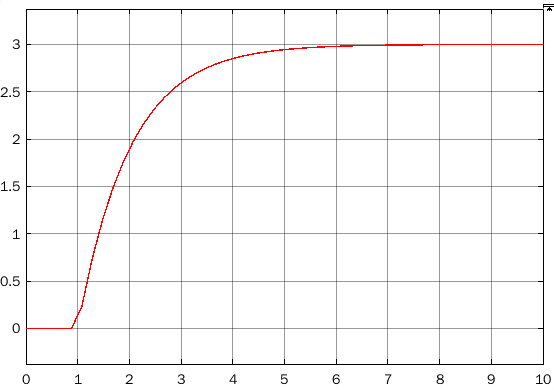
\includegraphics[width=\textwidth]{../assets/images/RTP/rtp_1_V13.png}
  \caption{SimuLink-Darstellung der Simulation für die Sprungantwort}
  \label{fig:rtp1v13}
\end{figure}

Wir erhalten aus der Simulation dann dieses Ergebnis:

\begin{figure}[h]
  \centering
  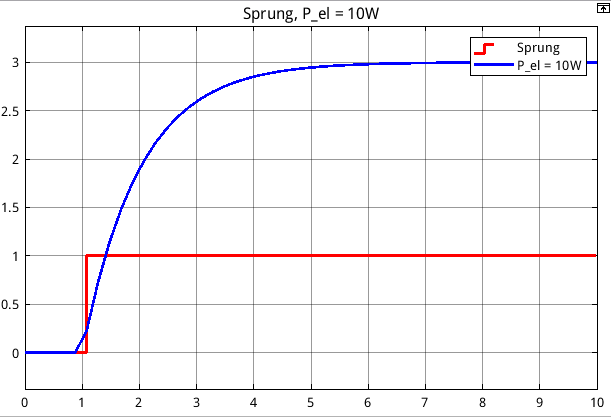
\includegraphics[width=\textwidth]{../assets/images/RTP/rtp_1_V13_2.png}
  \caption{Ergebnis der Simulation der Sprungantwort des Systems}
  \label{fig:rtp1v13_2}
\end{figure}

\newpage

\subsection{V1.4}

Wir wollen nun das oben verwendete Schaubild erweitern und verschiedene Temperaturanstiege als Antwort auf Sprünge in der Heizleistung $P_{th}$ darstellen.
\begin{table}[h]
  \centering
  \begin{tabular}{|c|c|}
    \hline
    $P_{0}$ & $\vartheta(t \to \infty)$\\
    \hline
    $10W$ & $3K$ \\
    $20W$ & $6K$ \\
    $30W$ & $9K$ \\
    \hline
  \end{tabular}
  \caption{Grenzwerte der Sprungantworten der Heizleitung $P_{el}$}
  \label{tab:limpel}
\end{table}

Wir erkennen nun auch den aus der Aufgabe V1.3 simulierten Endwert $y_{\vartheta}(t\to\infty) = 3K$. Mit der SimuLink erstellten Darstellung des Blockschaltbildes wollen wir nun mehrere gestreckte Sprünge darstellen:

\begin{figure}[h]
  \centering
  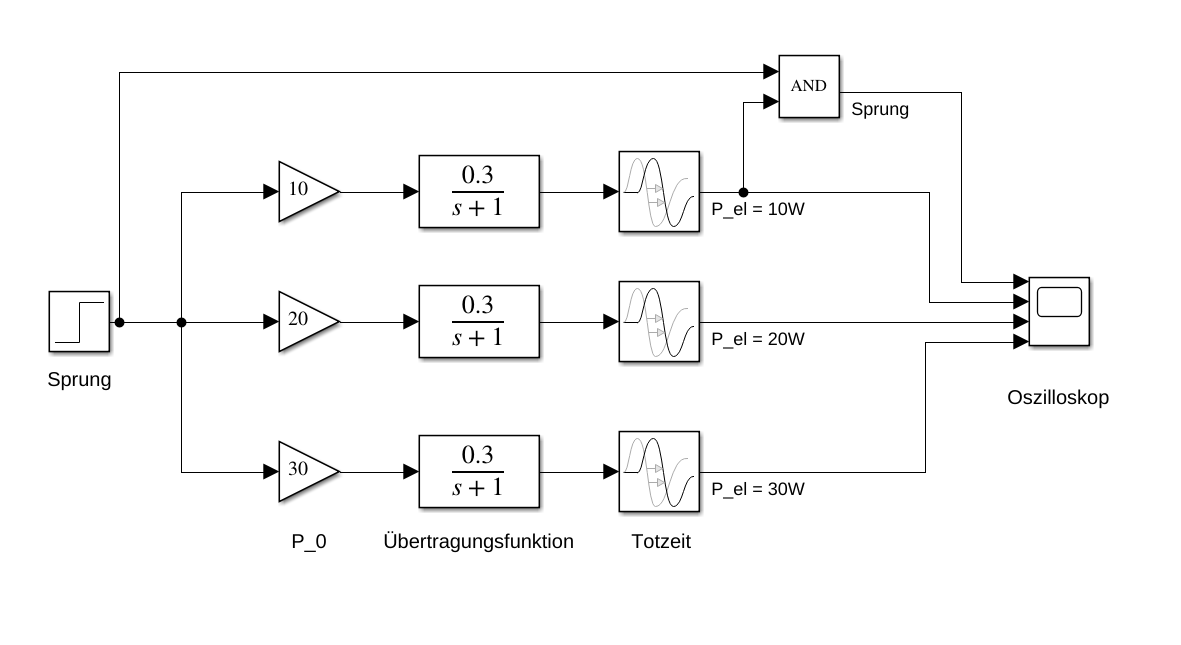
\includegraphics[width=\textwidth]{../assets/images/RTP/rtp_1_V14.png}
  \caption{SimuLink-Darstellung der Simulation aller drei Sprungantworten}
  \label{fig:rtp1v14}
\end{figure}

\newpage

Wir erkennen nun an dem Feld an Graphen, dass unsere vorher berechneten Grenzwerte korrekt sind. Physikalisch gesehen, erhöhen wir hier über die elektrische Leistung $P_{el}$ gleichzeitig die Heizleistung $P_{th}$. Damit wird die Luft in dem gleichen Zeitrahmen, da die Luft sich nicht schneller durch das Heizelement strömt, die Luft stärker, und kommt dementsprechend auch wärmer am Temperatursensor an. Es verändert sich dadurch allerdings nicht grundlegend die Eigenschaft des Systems.

\begin{figure}[h]
  \centering
  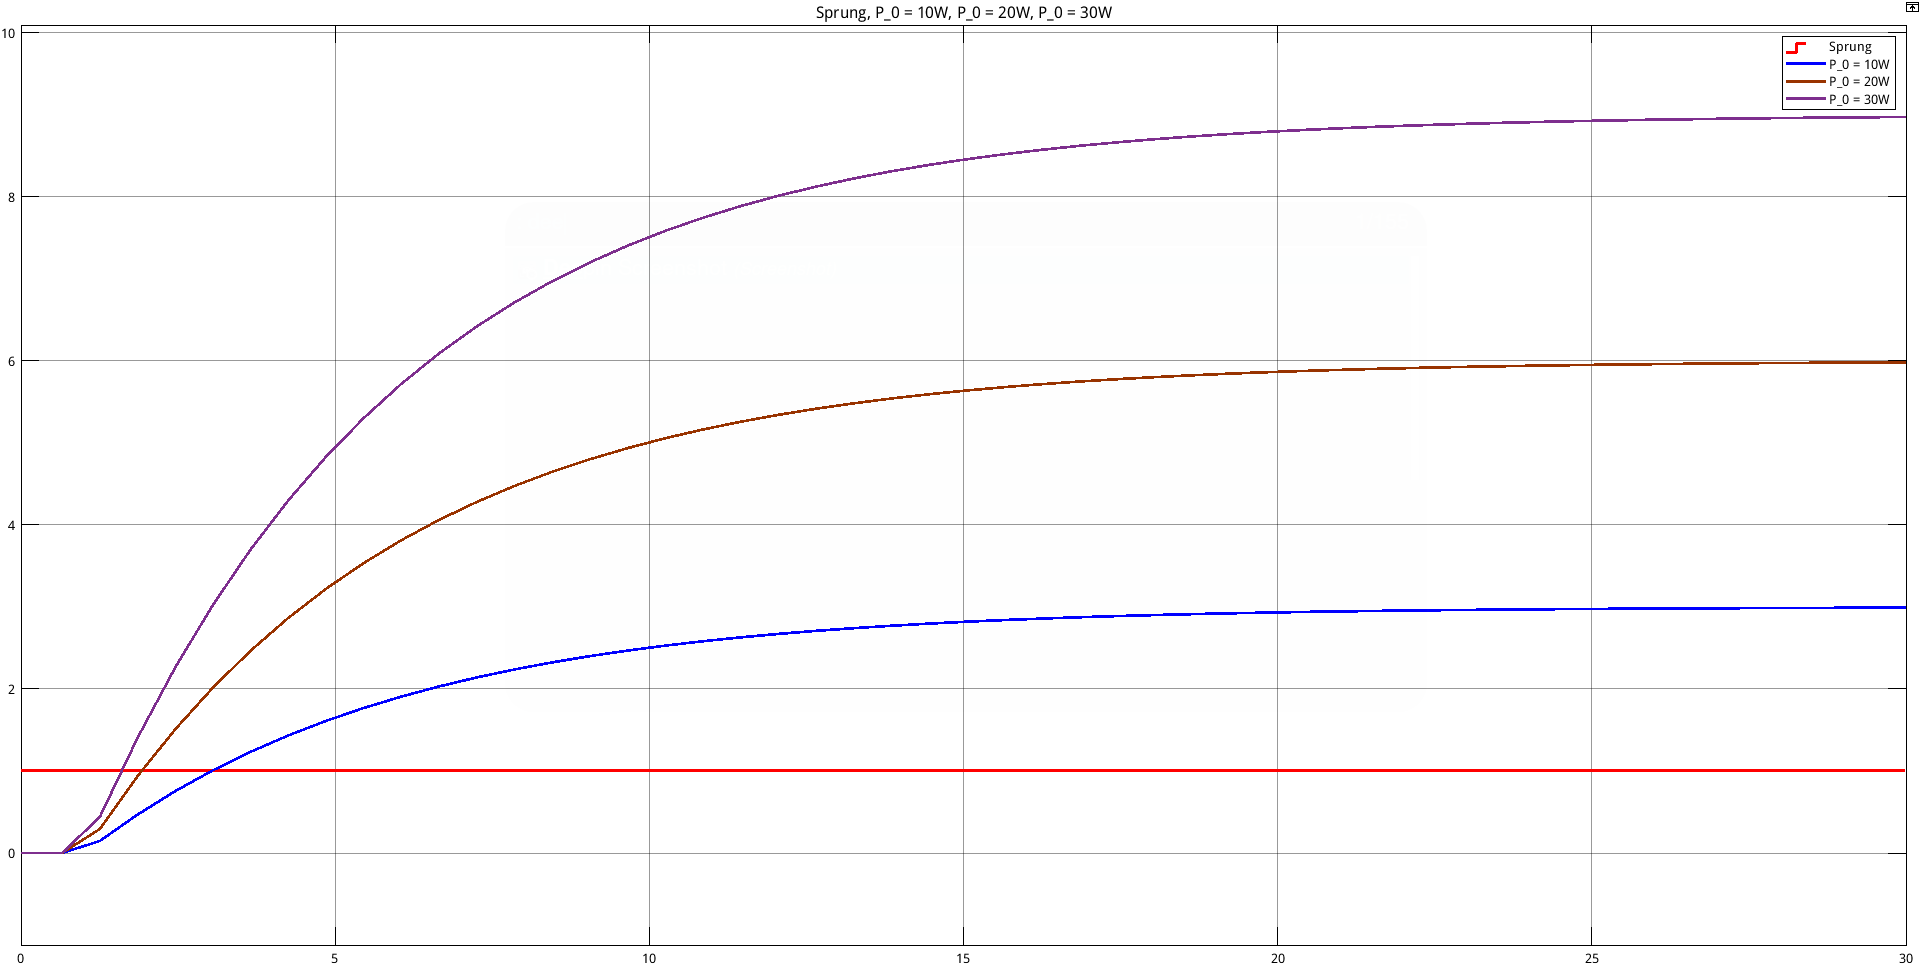
\includegraphics[width=\textwidth]{../assets/images/RTP/rtp_1_V14_2.png}
  \caption{Ergebnis der Simulation aller drei Graphen}
  \label{fig:rtp1v14_2}
\end{figure}

Auch hier erkennen wir das Totzeitglied $T_{t}$, auf welches die Heizleistung keinen Einfluss nimmt.

\newpage

\subsection{V1.5}

Als letzten Schritt unserer Vorbereitung möchten wir uns mit den Temperaturverläufen bei einem Sprung von $P_{el} = 10W\cdot \sigma(t)$ anschauen, wenn wir die Strömungsgeschwindigkeit $v$ variieren. Die Punkte, die wir uns dabei anschauen wollen, sind:

\begin{enumerate}[a)]
   \item $v = v_{L}$
   \item $v = \frac{v_{L}}{2}$
   \item $v = 2 \cdot v_{L}$
\end{enumerate}

Eine Änderung der Strömungsgeschwindigkeit hat einen Einfluss auf die folgenden Parameter:

\begin{align*}
  \label{eq:10}
  T_{s} &= \frac{C_{H}}{c_{L}\gamma_{L}Av}\\
  K_{s} &= \frac{1}{c_{L}\gamma_{L}Av}\\
  T_{t} &= \frac{l}{v}
\end{align*}

Wir berechnen nun für jeden Fall die entsprechenden Parameter und Grenzwerte und verwenden dann den Simulationsaufbau von V1.3, um die entsprechenden Graphen zeichnen zu können.

\begin{table}[h]
  \centering
  \begin{tabular}{|c||c|c|c|c|}
    \hline
    $v$ & $t_{t}$ & $K_{s}$ & $T_{s}$  & $\vartheta(t\to\infty)$\\
    \hline
    $v_{L}$ & $1s$ & $0,3\frac{K}{W}$ & $5s$ & $3K$ \\
    \hline
    $\frac{v_{L}}{2}$ & $2s$ & $0,6\frac{K}{W}$ & $10s$ & $6K$ \\
    \hline
    $2v_{L}$ & $0,5s$ & $0,15\frac{K}{W}$ & $2,5s$ & $1,5K$\\
    \hline
  \end{tabular}
  \caption{Auswirkung einer Änderung in der Strömungsgeschwindigkeit auf die Parameter}
  \label{tab:speed}
\end{table}
\newpage
Wir nutzen diese Werte um verschiedene Graphen mithilfe des folgenden Blockschaltbilds in SimuLink zu plotten:

\begin{figure}[h]
  \centering
  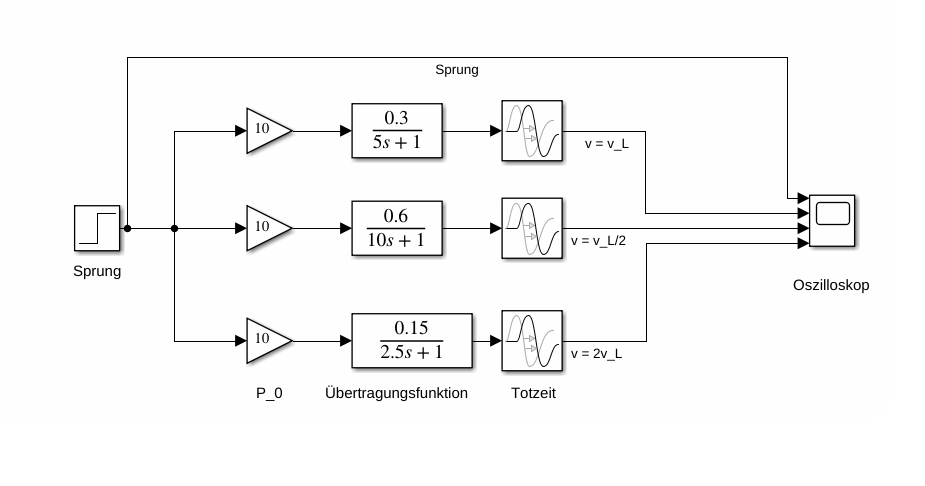
\includegraphics[width=0.8\textwidth]{../assets/images/RTP/rtp_1_V15.png}
  \caption{Blockschaltbild zur Simulation variabler Strömungsgeschwindigkeit $v_L$}
  \label{fig:vl}
\end{figure}
Wir bekommen dann folgende Simulationsergebnisse:

\begin{figure}[h]
  \centering
  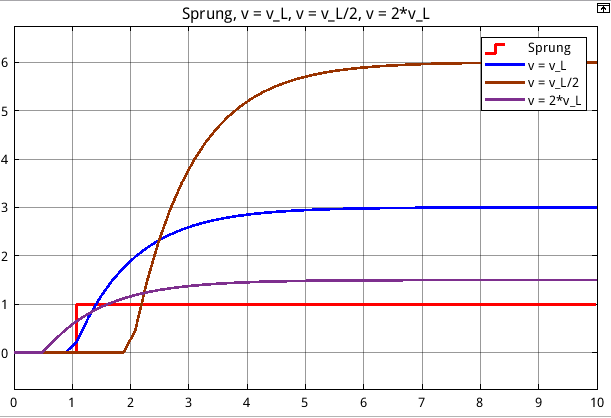
\includegraphics[width=0.8\textwidth]{../assets/images/RTP/rtp_1_V15_2.png}
  \caption{Simulationsergebnisse bei variabler Strömungsgeschwindigkeit $v_{L}$}
  \label{fig:vlplot}
\end{figure}

Unsere Erwartungen wurden bestätigt, da ein langsamerer Luftstrom zu einem längeren Zeitraum führt, in dem die Luft erwärmt werden kann. Außerdem dauert der Prozess nun länger und die Totzeit $T_{t}$ verlängert sich. Gleichzeitig führt ein schnellerer Luftstrom zu einer geringeren Erwärmung der Luft, dadurch dass sich die Luft kürzer aufwärmen kann, und zu einer kürzeren Totzeit, weil die Luft schneller durch das System strömt.

\newpage

\section{Auswertung}

\subsection{Stationäres Verhalten}
\label{sec:stat-verh}

Für die folgende Auswertung nehmen wir an, dass die Heizleitung $P_{el}$ proportional zur Heizungsansteuerung $u_{uP}$ und die Strömungsgeschwindigkeit der Luft $v_{L}$ proportional zur Lüfteransteuerung $u_{uL}$ ist. Ausgehend von der Gleichung \ref{eq:1} wollen wir nun die Kennlinienfelder zeichnen.
Zunächst wollen wir uns nun mit dem Kennlinienfeld $u_{y\vartheta} = f(u_{uP})$ mit $u_{uL} \in \{\text{4V, 5V, 6V}\}$ beschäftigen, dazu nehmen wir die Messwerte und tragen sie in unser Diagramm ein:

\begin{figure}[h]
  \centering
  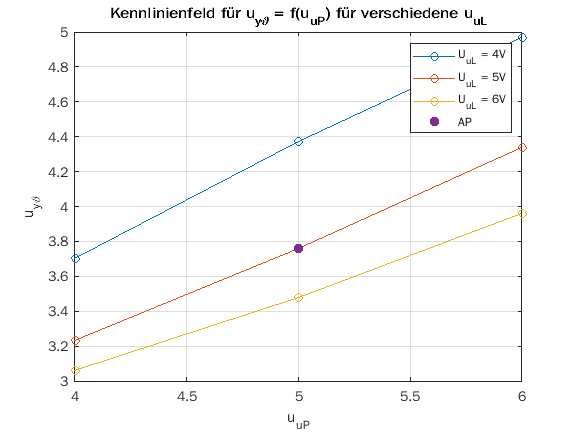
\includegraphics[width=0.8\textwidth]{../assets/images/RTP/kennlinieA11rtp1.png}
  \caption{Kennlinienfeld $f(u_{uP})$}
  \label{fig:kennuy}
\end{figure}

Gleichzeitig wollen wir uns nun auch das Kennlinienfeld zu $u_{y\vartheta} = f(u_{uL})$ mit $u_{uL} \in \{\text{4V, 5V, 6V}\}$ anschauen:

\begin{figure}[h]
  \centering
  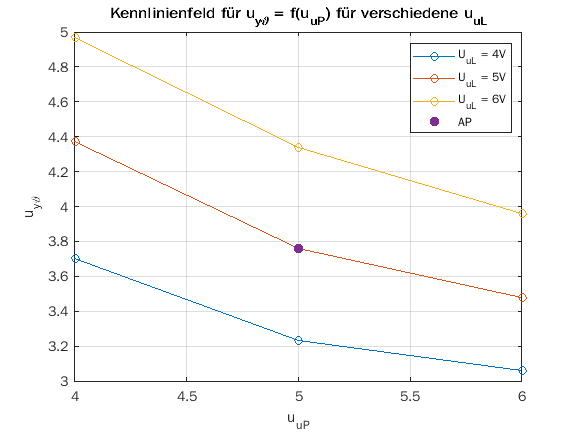
\includegraphics[width=0.8\textwidth]{../assets/images/RTP/kennlinieA12rtp1.png}
  \caption{Kennlinienfeld $f(u_{uL})$}
  \label{fig:kennux}
\end{figure}

In beiden Kennlinienfeldern wurde der Arbeitspunkt als violetter Punkt eingezeichnet.

Wri wollen uns nun einmal anschauen, wie die Spannungen $u_{uP}$ und $u_{y\vartheta}$ bei einer Temperatur von $\vartheta = 46^{\circ}C$ aussehen. Dazu berechnen wir zunächst die Messverstärkung

\begin{equation}
  \label{eq:12}
  K_{M} = \frac{\Delta u_{y\vartheta}}{\Delta \vartheta} = \frac{4,34V-3,23V}{44,3^{\circ}C-39,1^{\circ}C} \approx 0.213 \frac{V}{^{\circ}C}
\end{equation}

und berechnen nun den Spannungswert für $\vartheta = 46^{\circ}C$ über

\begin{equation}
  \label{eq:13}
  \Delta u_{y\vartheta} = K_{M} \cdot \Delta \vartheta = 0.213\frac{V}{^{\circ}C} \cdot (46^{\circ}C - 44.3^{\circ}C) = 0.36V
\end{equation}

Rechnen wir nun diesen Spannungswert $\Delta u_{y\vartheta}$ auf $u_{y\vartheta}$, so erhalten wir
\begin{equation}
  \label{eq:14}
  u_{y\vartheta}_{g} = \Delta u_{y\vartheta} + u_{y\vartheta} = 0.36V + 4.34V = 4.7V.
\end{equation}

Um nun noch auf $u_{uP}$ zu kommen, rechnen wir
\begin{equation*}
  \Delta u_{uP} = \frac{\Delta u_{y\vartheta}}{K_{ges}} = \frac{0.36V}{0.55} \approx 0.65V
\end{equation*}
also $u_{uP}_{g} = \Delta u_{uP} + u_{uP} = 0.65V + 6V = 6.65V$

Die Gesamtverstärkung des Systems
\begin{equation}
  \label{eq:11}
  K_{ges} = \frac{\Delta u_{y\vartheta}}{\Delta u_{uP}} = K_{u} \cdot K_{S} \cdot K_{M}
\end{equation}
setzt sich aus den Parametern

\begin{itemize}
  \item $K_{S} = \frac{\Delta \vartheta}{\Delta P_{el}}$

  \item $K_{u} = \frac{\Delta P_{el}}{\Delta u_{uP}}$ und
  \item $K_{M} = \frac{\Delta u_{y\vartheta}}{\Delta \vartheta}$
\end{itemize}
zusammen. Aus den Kennlinienfeld lässt sich nun die Gesamverstärkung als Steigung der mittleren, in rot markierten Gerade berechnen:

\begin{equation*}
  K_{ges} = \frac{\Delta u_{y\vartheta}}{\Delta u_{uP}} = \frac{4,34V - 3,23V}{6V-4V} = 0.55
\end{equation*}

\end{document}
